\documentclass[slovene,11pt,a4paper]{article}
\usepackage[margin=1.8cm,bottom=3cm,foot=1.5cm]{geometry}
\usepackage{amsmath}
\usepackage{booktabs}
\usepackage{float}
\usepackage{graphicx}
\usepackage{gensymb}
\usepackage{geometry}
\usepackage{changepage}
\usepackage{subcaption}
\usepackage{multirow}
\usepackage{blindtext}
\usepackage{hyperref}
\usepackage[version=4]{mhchem}
\usepackage[slovene]{babel}
\pagenumbering{gobble}
\renewcommand{\contentsname}{\centering Contents}

\begin{document}

\title{11. naloga - Optimalno filtriranje}
\author{Tadej Lozej 28201055}
\maketitle
\begin{center}
Modelska analiza 1 \\
\bigskip
Predavatelj: prof. dr. Simon Širca \\
Asistent: doc. dr. Miha Mihovilovič
\end{center}

\newpage

\tableofcontents

\newpage

\section{Uvod}

\pagenumbering{arabic}

Kadar z zaporednimi meritvami spremljamo časovni razvoj procesa, katerega dinamiko poznamo, lahko s filtriranjem dosežemo boljšo natančnost, kot jo dajejo surove meritve. Kalmanov filter deluje na principu optimalnega uteževanja linearne napovedi stanja ter novih meritev, kar doseže s sprotnim vodenjem evidence o kovarianci trenutne ocene stanja.

Naj bo $\vec{x}_n$ vektor stanja sistema od času $n$, $P_n$ pa pripadajoča kovariančna matrika, ki opisuje njegovo statistično negotovost. Potrebujemo še začetno stanje $\vec{x}_0^+$ ter kovarianco $P_0^+$, ki ju običajno dobimo iz prve surove meritve. Komponentam stanja, ki niso na voljo nastavimo velike začetne kovariance.

Kalmanov filter poteka v dveh korakih. Prvi korak je izvedba časovnega koraka na trenutni napovedi stanja. Fizikalni sistem naj uboga časovno evolucijo $\vec{x}_{n+1} = F_n \vec{x}_n + \vec{c}_n + \vec{w}_n$, kjer je $F_n$ prehodna matrika sistema, $\vec{c}_n$ kontrolni vektor, $\vec{w}_n$ pa vektor Gaussovega šuma s povprečjem $0$ in kovariančno matriko $Q_n$. Napovemo novo stanje $\vec{x}_{n+1}^-$ ter njegovo kovariančno matriko $P_{n+1}^-$:

\begin{align}
\vec{x}_{n+1}^- &= F_n \vec{x}_n^+ + \vec{c}_n, \\
P_{n+1} &= F_n P_n^+ F_n^T + Q_n.
\end{align}
Sledi izboljšava te napovedi z meritvamni. V splošnem ne merimo neposredno komponent vektorja stanja $\vec{x}_n$, temveč neko linearno kombinacijo $\vec{z}_n = H_n \vec{x}_n + \vec{r}_n$, kjer je $H_n$ matrika, ki določa, kaj merimo, $\vec{r}_n$ pa šum meritve s kovariančno matriko $R_n$. Matrika $H_n$ je lahko singularna, če merimo manj spremenljivk, kot je dimenzija sistema.

\begin{align}
K_{n+1} &= P_{n+1}^- H_{n+1}^T ( H_{n+1} P_{n+1}^- H_{n+1}^T + R_{n+1})^{-1}, \\
\vec{x}_{n+1}^+ &= \vec{x}_{n+1}^- + K_{n+1}(\vec{z}_{n+1} - H_{n+1}\vec{x}_{n+1}^-, \\
P_{n+1}^+ &= (I-K_{n+1}H_{n+1}) P_{n+1}^-.
\end{align}
Prva enačba določa izboljšanje natančnosti stanja zaradi novih meritev, $K_{n+1}$ je pa faktor ojačanja, ki določa, s kolikšno utežjo nova meritev prispeva k popravku.

\section{Rekonstrukcija poti vozila}

Tipičen primer uporabe Kalmanovega filtra je rekonstrukcija poti in hitrosti vozila na podlagi GPS podatkov o lokaciji, sprotnih podatkov o hitrosti vozila ter pospeškov z akcelometra. V datoteki \texttt{kalman\_cartesian\_data.dat} na spletni strani predmeta Modelska analiza 1 so po stolpcih podani čas $t$, zašumljene meritve položaja $(x_n, y_n)$, hitrosti $(v_{x,n}, v_{y,n})$ ter pospeškov $(a_{x,n}, a_{y,n})$. Eksaktne vrednosti položajev in hitrosti za kontrolo pravilnosti najdemo v datoteki \texttt{kalman\_cartesian\_kontrola.dat}. Vse količine so v osnovnih SI enotah.

Na sliki 1 so na zgornjem grafu prikazane meritve ter eksaktne vrednosti (kontrola) lokacije po poti od Ljubljane do Litije, na spodnjem pa meritve ter eksaktne vrednosti komponent hitrosti. Na zgornjem grafu je prikazano tudi povečano krožišče. Na povečavi bolje vidimo razpršenost meritev okrog eksaktne lege.

\begin{figure}[h!]
\centering
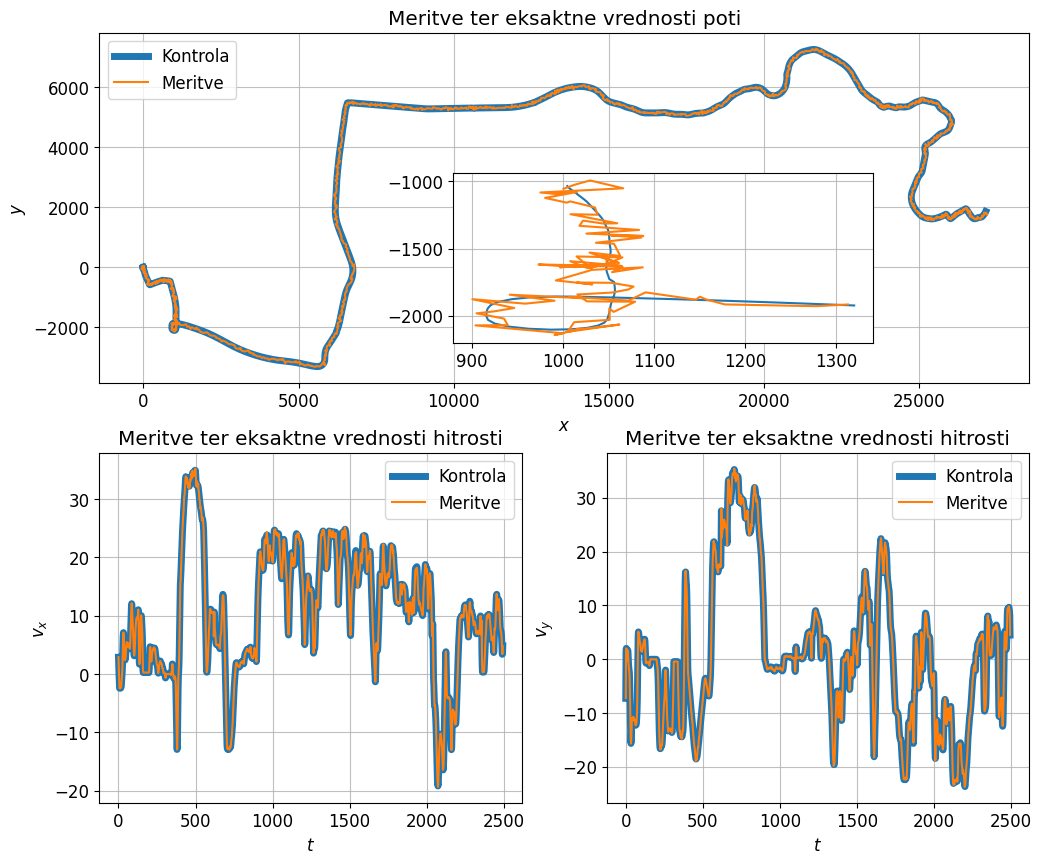
\includegraphics[width=14cm]{slika1.png}
\caption{Meritve z oranžno črto ter eksaktne vrednosti poti z odebeljeno modro črto. Vidimo raztresenost meritev okrog eksaktne vrednosti ter upamo, da nam bo filter pomagal in zgladil pot.}
\end{figure}

Konstruirajmo Kalmanov filter za naš primer. Vektor stanja je $\vec{x} = (x,y,v_x,v_y)$, kontrolni vektor pa dobimo iz pospeška, $\vec{c} = (a_x \Delta t^2 / 2, a_y \Delta t^2 / 2, a_x \Delta t, a_y \Delta t)$. Prehodna matrika sistema je konstantna in izhaja iz kinematičnih zvez

\[ F = 
\begin{bmatrix}
 I_{2\times 2} & I_{2\times 2}\Delta t \\
 0 & I_{2\times 2},
\end{bmatrix}
\]
šum časovne evolucije sledi iz pospeška, $Q_n = \text{diag}(\sigma_a^2 \Delta t^4 / 4, \sigma_a^2 \Delta t^4 / 4, \sigma_a^2 \Delta t^2, \sigma_a^2 \Delta t^2)$, šum meritev pa iz napak GPS podatkov ter hitrosti $R_n = \text{diag}(\sigma_{xy}^2,\sigma_{xy}^2, \sigma_{v}^2, \sigma_{v}^2)$.

Podatki so vzorčeni vsakih $\Delta t = 1.1783 \, \text{s}$. Za pospeške sta znani absolutni napaki $\sigma_{xy} = 25 \, \text{m}$, $\sigma_a = 0.25 \, \text{ms}^{-2}$, za hitrost pa poznamo relativno napako $\sigma_v = 0.01||\vec{v}||$, pri čemer napako vseeno navzdol omejimo na $1 \, \text{km/h}$.

Na sliki 2 so z zeleno črto prikazani rezultati dobljeni s Kalmanovim filtrom, kjer smo upoštevali vse meritve. Vidimo, da so rezultati precej dobri. Predvsem zgladijo pot iz zašumljenih podatkov. To lahko zelo očitno vidimo na zgornjem grafu pri povečanem odseku s krožiščom.

\begin{figure}[h!]
\centering
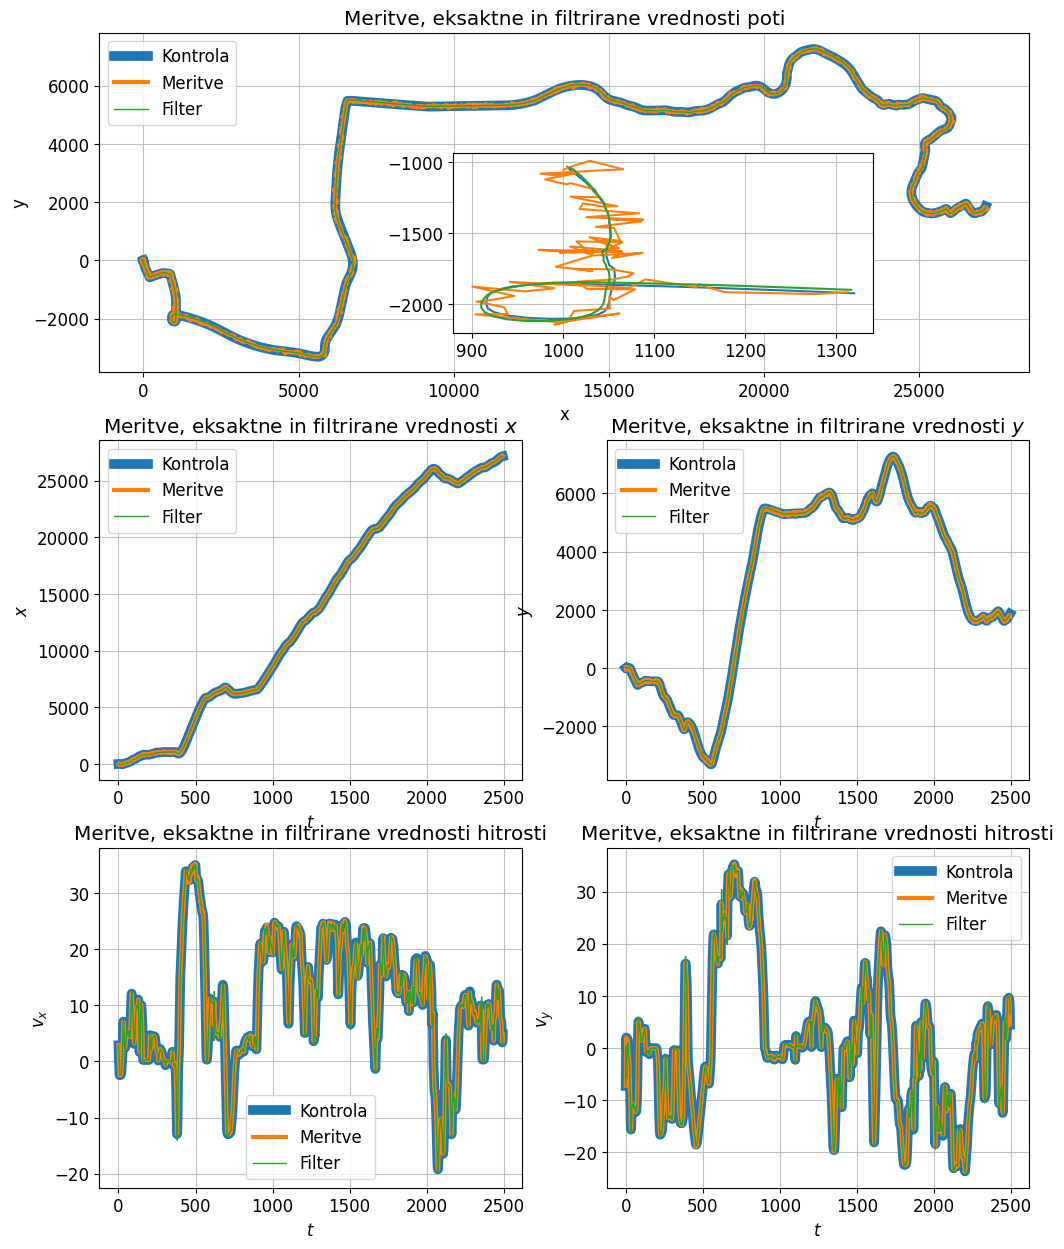
\includegraphics[width=14cm]{slika2.png}
\caption{Rekunstrukcija poti ter hitrosti s Kalmanovim filtrom z zeleno črto. Na grafih so prikazani tudi kontrolni podatki z odebeljeno modro črto ter meritve z oranžno črto. Na podrobneje prikazanemo krožišču vidimo kako filter zgladi pot iz vhodnih meritev.}
\end{figure}

Zanima nas tudi natančnost filtra seveda. Na sliki 3 so prikazana odstopanja krajevnih in hitrostnih koordinat od kontrolnih vrednosti v odvisnosti od časa. Na grafih je prikazano odstopanje filtra, kjer upoštavamo vse izmerjene meritve ter odstopanje filtra pri katerem upoštevamo le vsako peto meritev hitrosti in vsako deseto meritev lokacije. Kot notacijo bom uporabljal Filter($i$,$j$), kjer bo $i$ korak vzorčenja lokacije ter $j$ korak vzorčenja hitrosti. Kot pričakovano vidimo, da so načeloma napake filtra kjer upoštevamo vse meritve manjše kot napake filtra, kjer upoštevamo le vsako deseto meritev lokacije ter vsako peto meritev hitrosti. Treba je pa poudariti, da tudi v drugem primeru filtra napake niso velike! To, da upoštevamo le vsako $i$-to meritev lokacije ter vsako $j$-to meritev hitrosti dosežemo z matriko $H$. Matrika $H$ je v našem primeru diagonalna, saj ni med merjenimi ter želenimi količinami nobene transformacije. Na diagonalo postavimo vrednost 1, če meritev želimo upoštevati ali vrednost 0, če meritve ne želimo upoštevati. Glede na našo konstrukcijo filtra prva dva diagonalca v matriki $H$ določata upoštevanje krajevnih koordinat ($x$, $y$), zadnja dva diagonalca pa določata upoštevanje hitrostnih koordinat ($v_x$, $v_y$).

\begin{figure}[h!]
\centering
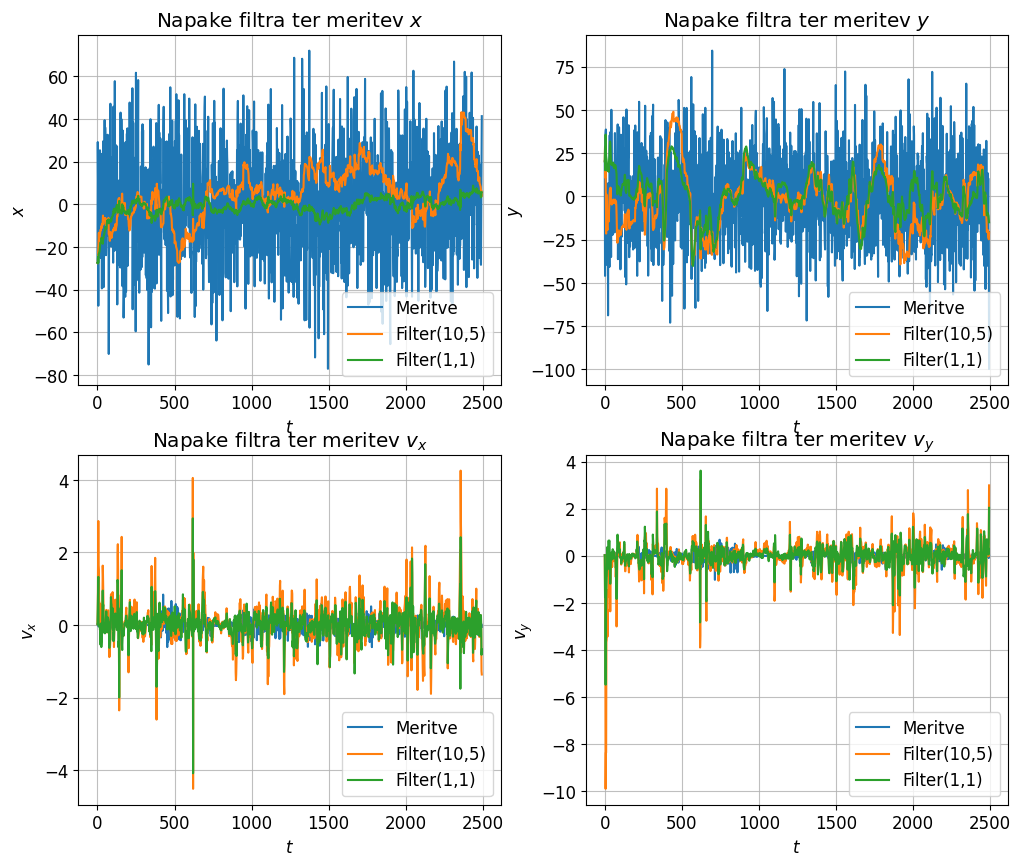
\includegraphics[width=14cm]{slika3.png}
\caption{Napake količin dobljenih s Kalmanovim filtrom. Pri filtru Filter(1,1) smo upoštevali vse meritve pri črti Filter(10,5) pa vsako deseto meritev lokacije ter vsako peto meritev hitrosti.}
\end{figure}

Na sliki 4 je prikazana evklidska razdalja med vektorjema $\vec{x}_n^+$ ter $\vec{x}_n^-$ za Filter(1,1) ter Filter(10,5) v logaritemski skali. Ko napoved popravimo, se pravi ko upoštevamo meritev, v povprečju bolj popravimo napoved pri filtru Filter(10,5). V prejšnjem stavku je pomembno, da gledamo le vektorje pri časovnih značkah ko napoved popravimo, saj pri filtru Filter(1,1) napoved popravimo pri vsaki časovni znački, medtem ko pri filtru Filter(10,5) popravimo napoved z upoštevanjem meritve le pri vsaki peti časovni znački, saj takrat dobimo novo meritev.

\begin{figure}[h!]
\centering
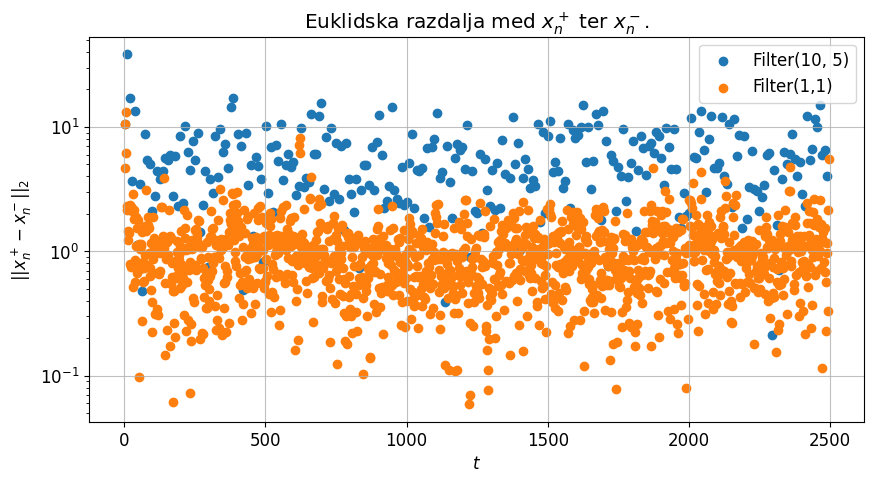
\includegraphics[width=12cm]{slika4.png}
\caption{Evklidska razdalja med prvotno oceno stanja sistema ter izboljšano oceno stanja sistema po dobljeni meritvi za filter pri katerem upoštevamo vsako meritev ter za filter pri katerem upoštevamo vsako deseto meritev lokacije ter vsako peto meritev hitrosti.}
\end{figure}

Z kalmanovim filtrom poleg ocen za željene količine spremljamo tudi oceno za konariančno matriko skupaj s časom. Neničelni elementi kovariančne matrike z našim filtrom so prikazani na sliki 5. Tukaj imamo z modro, zeleno in oranžno polno črto prikazane elemente $\sigma_{xy}^2$, $\sigma_{v}^2$ ter $\sigma_{(xy),v}$ kovariančne matrike $P^+$ filtra Filter(10,5) ter z rdečo, vijolično ter rjavo črtkano črto prikazane enake elemente kovariančne matrike $P^+$ filtra Filter(1,1). Vidimo, da so elementi kovariančne matrike pri filtru Filter(1,1) manjši kot elementi kovariančne matrike pri filtru Filter(10,5). Krajevne koordinate lahko v enem primeru določimo na približno $10 \, \text{m}$ natančno, medtem ko jih v drugem primeru lahko določimo z natančnostjo $\sqrt{10} \, \text{m} \approx 3,2 \, \text{m}$.Prav tako se na grafu zelo lepo vidi kje v filtru Filter(10,5) pridobimo nove meritve, saj takrat konarianca očitno pade in dobimo nekako žagast graf. Prvi vrh pri negotovosti  se pojavi malo pred časom $t = 500 \, \text{s}$. Ob tem času se nahajamo na avtocesti po rondoju. Verjetno do negotovosti pride zaradi velikih hitrosti in posledično bolj redkega vzorčenja v krajevnem smislu. Druga dva vrhova pa se pojavita v časih okrog $t = 750 \, \text{s}$ in sodita k ovinkom na avtocesti pri $(x,y) \approx (6750 \, \text{m}, 0 \, \text{m})$ ter $(x,y) \approx (6200 \, \text{m}, 2000 \, \text{m})$. V teh ovinkih je namreč hitrost precej visoka in podatki precej raztreseni. Mogoče v teh delih celo vozimo skozi tunele.

\begin{figure}[h!]
\centering
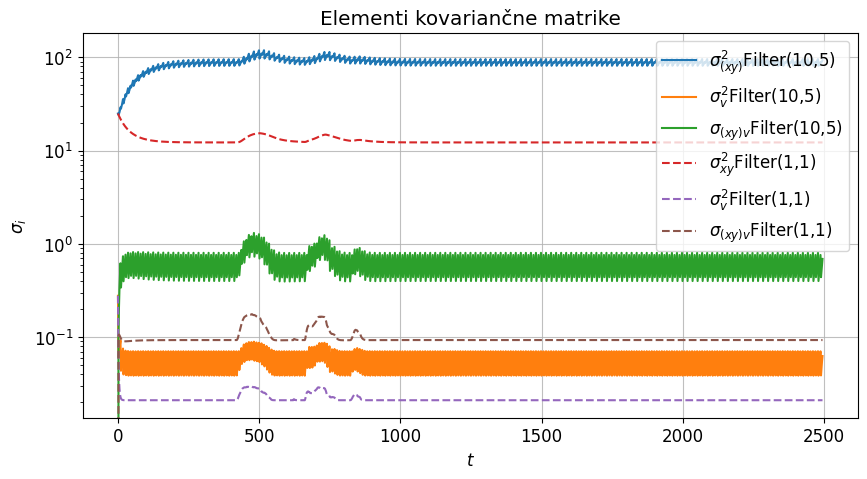
\includegraphics[width=12cm]{slika5.png}
\caption{Elementi kovariančne matrike $P^+$ za filtra Filter(1,1) in Filter(10,5). Vidimo, da so kovariance filtra Filter(1,1) manjše. Kovariance Filtra(10,5) so v času žagaste zaradi upoštevanja novih podatkov vsak peti korak. Vrhovi v kovariancah ustrezajo ovinkom na avtocesti.}
\end{figure}

Za analizo natančnosti časovne vrste si izberimo RMSE metriko. Definirana je kot

\begin{equation}
\text{RMSE} = \sqrt{\sum_t (\hat{x}-x})^2, 
\end{equation}
kjer je $\hat{x}$ naša ocena oz. napoved za spremenljivko $x$ pa njena dejanska vrednost. Vsota teče po času. To je v resnici seveda koren povprečnega odstopanja kvadrata. Oglejmo si vrednost RMSE metirke v odvisnosti od $(i,j)$, se pravi pogostosti vzorčenja krajevnih ter hitrostnih koordinat v tem vrstnem redu. Rezultati so prikazani na sliki 6. Očitno več podatkov kot damo filtru boljši je. Zanimivo je pa videti, da na prvi pogled se napovedi krajevnih koordinat hitreje slabšajo v smeri naraščajočega $i$. V skladu s tem lahko sklepamo, da k natančnejši napovedi krajevnih koordinat prispevajo podatki o krajevnih koordinatah več kot podatki o hitrostnih koordinatah. Obratno velja za hitrostne koordinate. Poglejmo si kako filter nastopi, če enih ali drugih koordinat nimamo na voljo.

\newpage

\begin{figure}[h!]
\centering
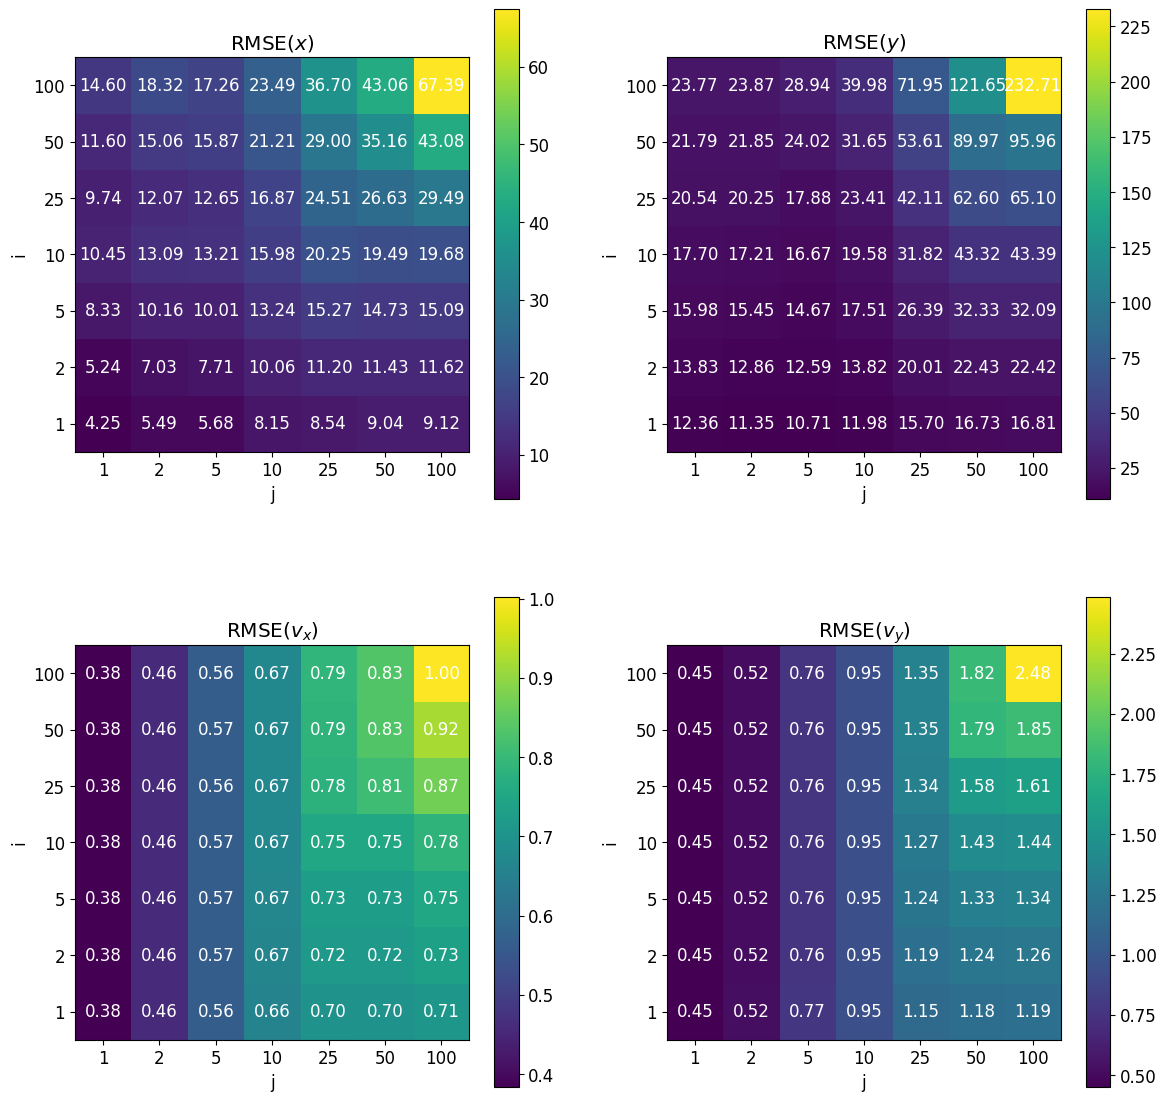
\includegraphics[width=14cm]{slika6.png}
\caption{RMSE vrednosti za različne kalmanove filtre ($i$,$j$). Sklepamo, da k natančnejši napovedi krajevnih koordinat prispevajo podatki o krajevnih koordinatah več kot podatki o hitrostnih koordinatah. Obratno velja za hitrostne koordinate.}
\end{figure}


\subsection{Rekonstrukcija poti vozila brez podatkov o hitrosti ali položaju.}

Poglejmo kako dobro lahkos kalmanovim filtrom napovemo željene količine brez meritev hitrosti ali položaja. V problemu uporabljamo isti filter kot prej, le da podatkov o hitrosti oz. položaju ne zajemamo. V matriki $H$ sta tako zadnja dva oz. prva dva diagonalca vedno enaka 0. Na sliki 7 si poglejmo vizualno rekonstrukcijo poti ter eksaktne, merjene ter filtrirane vrednosti opazovanih količin. Vidimo, da je filter brez hitrosti na več odsekih precej nenatančen. Predvsem ga motijo ovinki. Tudi v približanem krožišču vidimo, da filter precej odmaknjen od kontrolnih vrednosti. Največja zmota je pa takoj na začetku v smeri $y$ ter tudi v tej komponenti hitrosti posledično. Vseeno pa izgleda filter brez hitrosti na prvi pogled vsaj v ovinku boljši kot filter brez položaja, ki ima očitno nek konstanten odmik od pravih vrednosti krajevnih koordinat. Medtem, ko se filter brez hitrosti trudi ujeti pravo pot je filter brez položaja že neopravičljivo samozavesten.

\begin{figure}[h!]
\centering
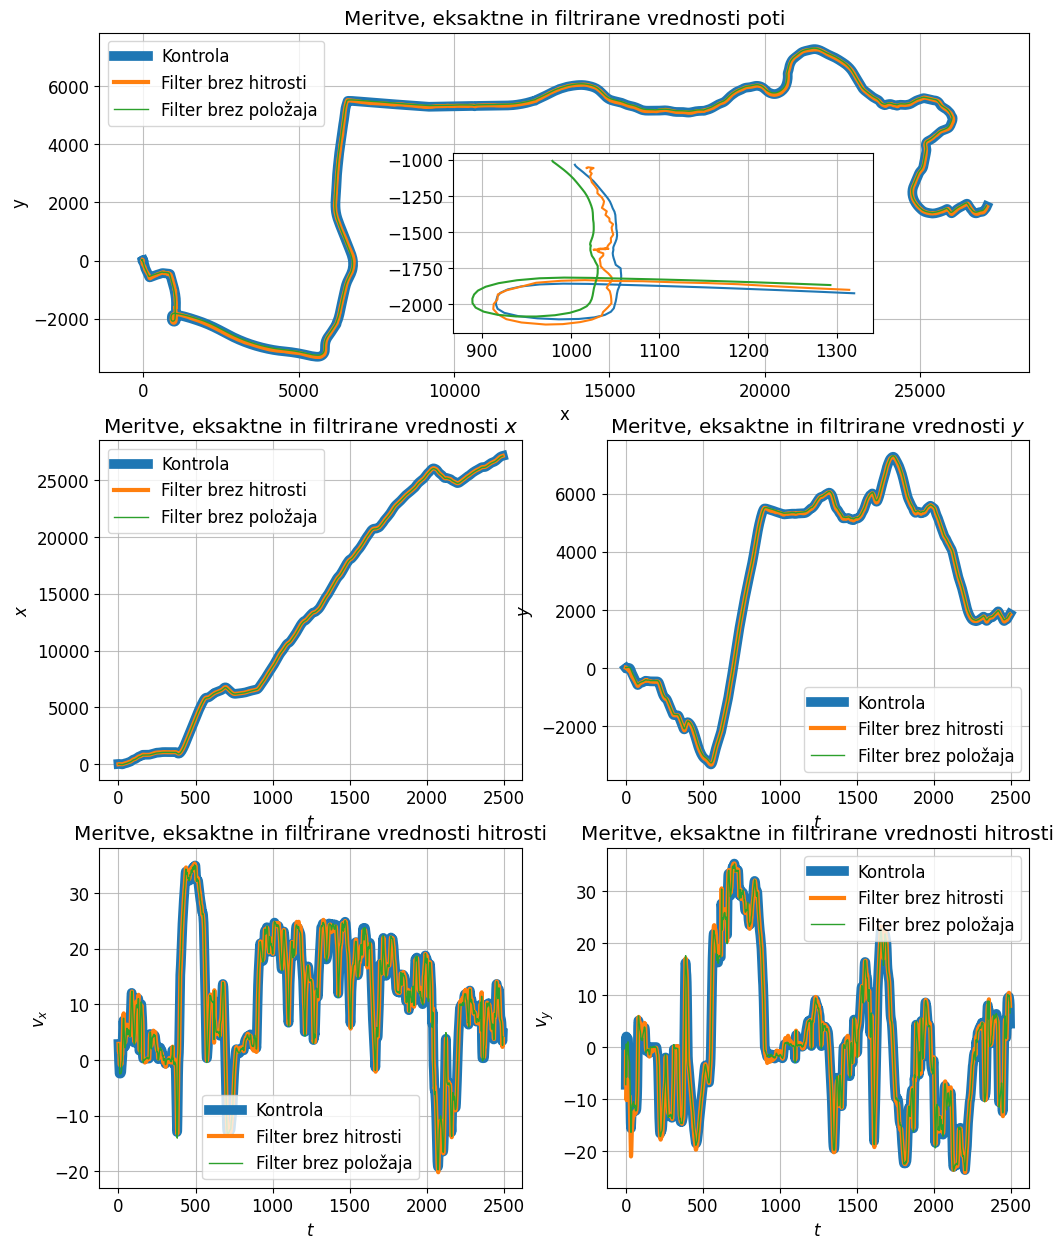
\includegraphics[width=14cm]{slika7.png}
\caption{Rekunstrukcija poti ter hitrosti s Kalmanovim filtrom brez podatkov o hitrosti z oranžno črto ter Kalmanovim filtrom brez podatkov o položaju z zeleno črto. Na grafih so prikazani tudi kontrolni podatki z odebeljeno modro črto. Na podrobneje prikazanemo krožišču vidimo kako se filter brez hitrosti trudi ujeti kontrolne podatke ter kako filter brez položaja samozavestno napoveduje s konstantnim zamikom od kontrolnih vrednosti.}
\end{figure}

Na sliki 8 so prikazane napake krajevnih ter hitrostnih koordinat v odvisnosti od časa. Vidimo, da so te napake večje kot, če filtru podajamo obojne podatke. To 
se sploh vidi pri oceni hitrostnih koordinat za filter brez podanih hitrosti in pri oceni krajevnih koordinat za filter brez podanega položaja. V smeri $y$ se pri položaju zmotimo tudi do $100 \, \text{m}$ takoj na začetku našega potovanja in pri hitrosti ob istem času za $10 \, \frac{\text{m}}{\text{s}}$, kar je $36 \, \frac{\text{km}}{\text{h}}$! Na prvem grafu na sliki vidimo zelo očiten konstanten zamik krajevne koordinate $x$, ki ga filter ne zna popraviti. Prav tako pri drugi krajevni koordinati vidimo konstanten zamik, le da je ta bolj zašumljena. Kot pričakovano pa seveda hitrosti bolje napove filter, ki mu tudi podajamo podatke o hitrosti, se pravi filter brez podatkov  položaja.

\begin{figure}[h!]
\centering
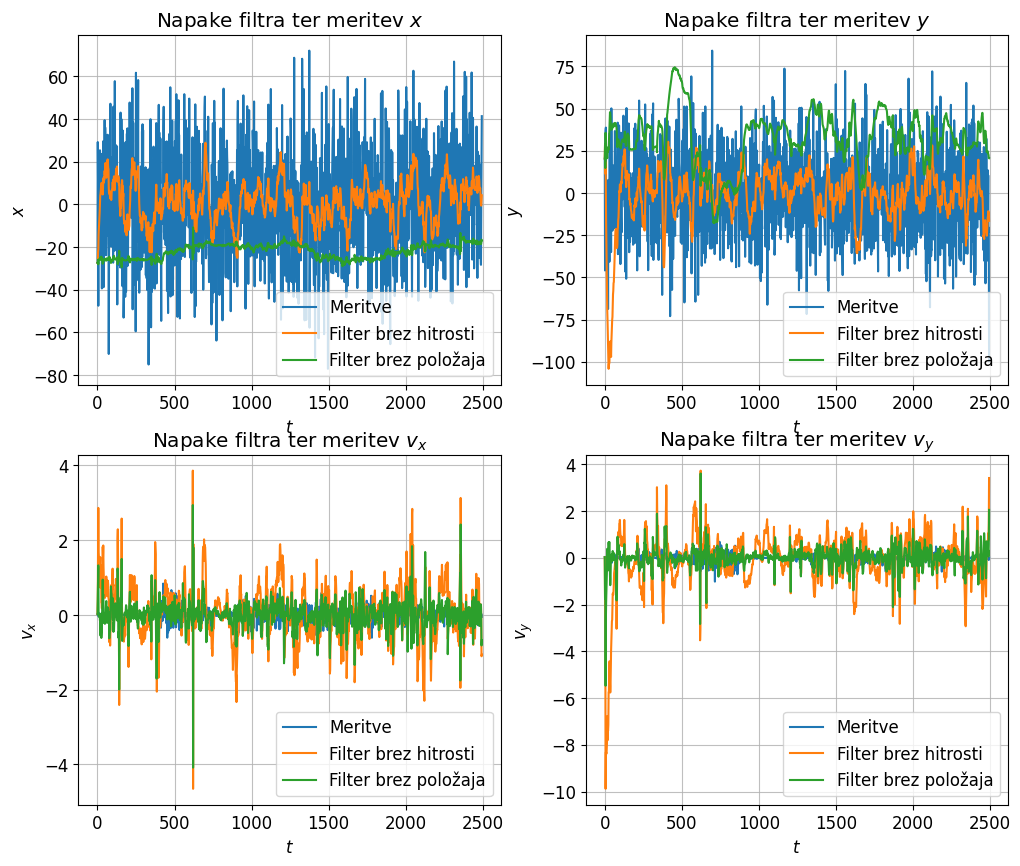
\includegraphics[width=14cm]{slika8.png}
\caption{Napake količin dobljenih s Kalmanovim filtrom brez podatkov o hitrosti ter Kalmanovim filtrom brez podatkov o položaju.}
\end{figure}

Na sliki 9 so prikazani elementi kovariančne matrike $P^+$ za Kalmanov filter brez podatkov o hitrosti in Kalmanov filter brez podatkov o položaju. Vidimo, da so kovariance količin večje kot v primerih, kjer filtru podajamo obojne podatke. Pri tem grafu lahko komentiramo to, da je pri filtru brez hitrosti kovariancam ne pozna več treh lokalnih maksimumov pri časih $t\approx 500 \, \text{s}$, $t\approx 700 \, \text{s}$ ter $t\approx 800 \, \text{s}$. Pri filtru brez položaja nas pa zaskrbi kovarianca položaja, saj ta nenehno narašča, medtem ko se druge kovariance ustalijo pri nekih vrednostih.

\begin{figure}[h!]
\centering
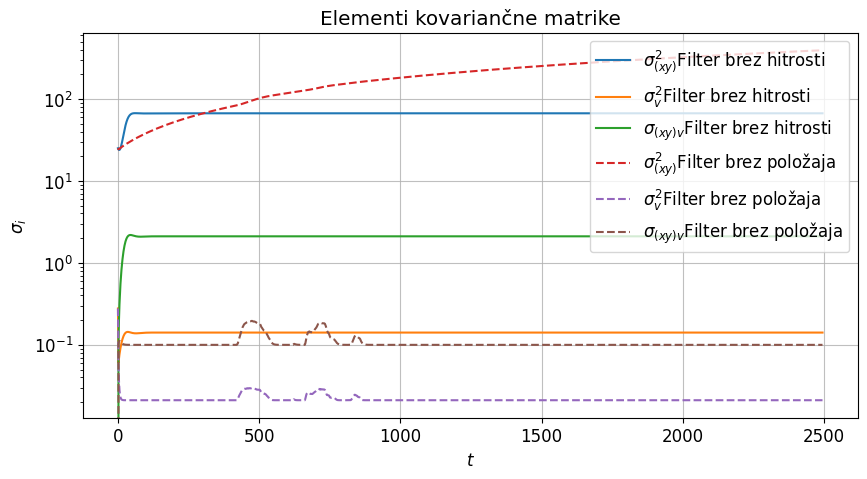
\includegraphics[width=12cm]{slika9.png}
\caption{Elementi kovariančne matrike $P^+$ za Kalmanov filter brez podatkov o hitrosti s polnimi črtami ter elementi kovariančne matrike $P^+$ za Kalmanov filter brez podatkov o položaju. Vidimo, da kovarianca položaja za filter brez hitrosti konstantno narašča, medtem, ko se druge ustalijo pri nekih vrednostih.}
\end{figure}

Slika 10 prikazuje RMSE vseh gledanih krajevnih ter hitrostnih koordinat filtra brez hitrosti s polno modro črto ter filtra brez položaja s črtkano oranžno črto v odvisnosti od koraka s katerim jemljemo krajevne podatke $i$ oz. hitrostne podatke $j$. Vidimo, da RMSE krajevnih koordinat pri filtru brez hitrosti zašumljeno in strmo narašča. V hitrostnih koordinatah se pa filtra po nekaj vrednostih $i$ oz. $j$ ujameta.

\newpage

\begin{figure}[h!]
\centering
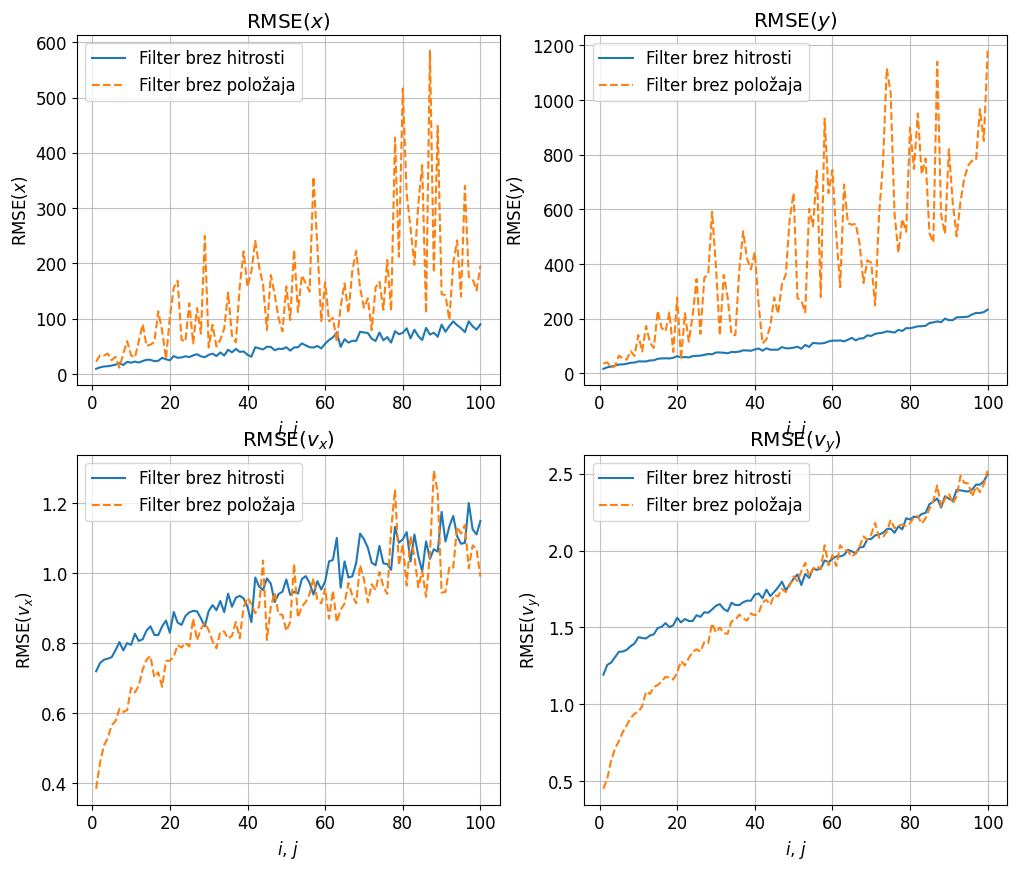
\includegraphics[width=12cm]{slika10.png}
\caption{Elementi kovariančne matrike $P^+$ za Kalmanov filter brez podatkov o hitrosti.}
\end{figure}

\subsection{Rekonstrukcija poti iz radialnega in tangencialnega pospeška}

V resnici nam akcelometer podaja pospeške $\vec{a} = (a_t, a_r)$ glede na trenutno orientacijo vozila. Med kontrolnim vektorjem in nehomogenim delom dinamičnega modela zato stoji še ena linearna preslikava $B_n: \, \vec{c}_n = B_n \vec{u}_n$. V tem primeru gre za ortogonalno transformacijo, definirano s trenutno oceno hitrosti:

\begin{equation}
\vec{u}_n  = (\vec{a}_n \Delta t**2 /2, \vec{a}_n \Delta t), \quad
B_n = 
\begin{bmatrix}
 B_n^{vv} & 0 \\
 0        & B_n^{vv}
\end{bmatrix}
,\quad
B_n^{vv} = \frac{1}{||\vec{v}_n||}
\begin{bmatrix}
 v_x & -v_y \\
 v_y & v_x
\end{bmatrix}
\end{equation}
Drugi člen v hitrostno-hitrostnem bloku $Q_n^{vv}$ mi je delal težave in sem ga zato izpustil. Ne poznamo tudi začetne hitrosti, zato sem za začetno hitrost dal neko majhno vrednost z veliko kovarianco. Rezultati poti dobljene z relativnim filtrom so prikazani na sliki 11.

\begin{figure}[h!]
\centering
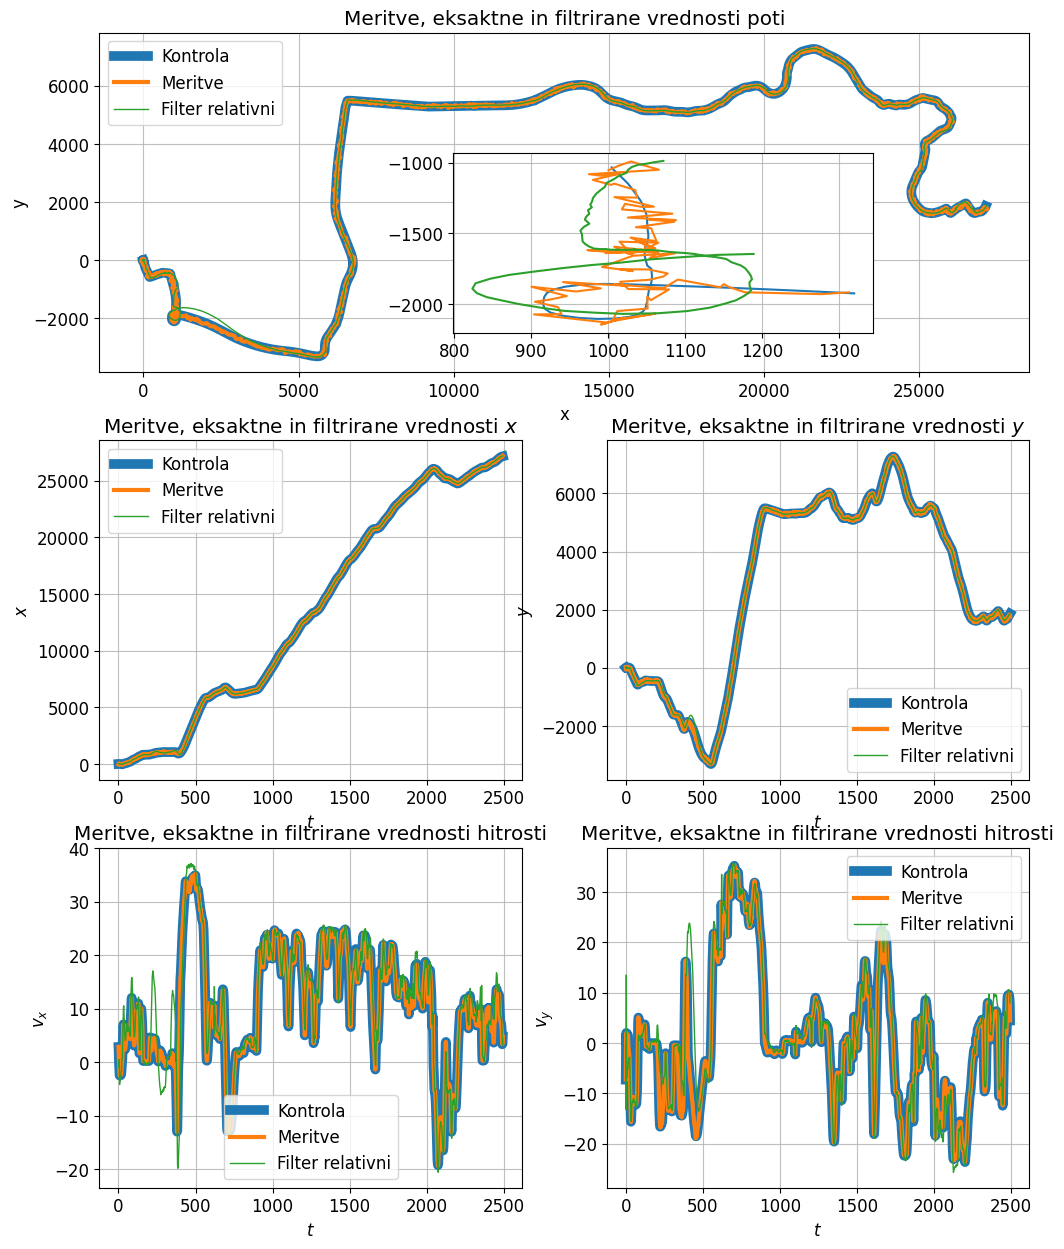
\includegraphics[width=14cm]{slika11.png}
\caption{Rekunstrukcija poti ter hitrosti s Kalmanovim filtrom z relativnimi podatki o pospeških z zeleno črto. Na grafih so prikazani tudi kontrolni podatki z odebeljeno modro črto ter meritve z oranžno črto. Na podrobneje prikazanemo krožišču vidimo kako oddaljen je filter od kontrolne poti.}
\end{figure}

Na sliki 12 so nato prikazane še napake relativnega ter katerzičnega filtra v odvisnosti od časa. Vidimo, da se po nekaj časa tudi relativen filter ujame in nastopi precej dobro.

\begin{figure}[h!]
\centering
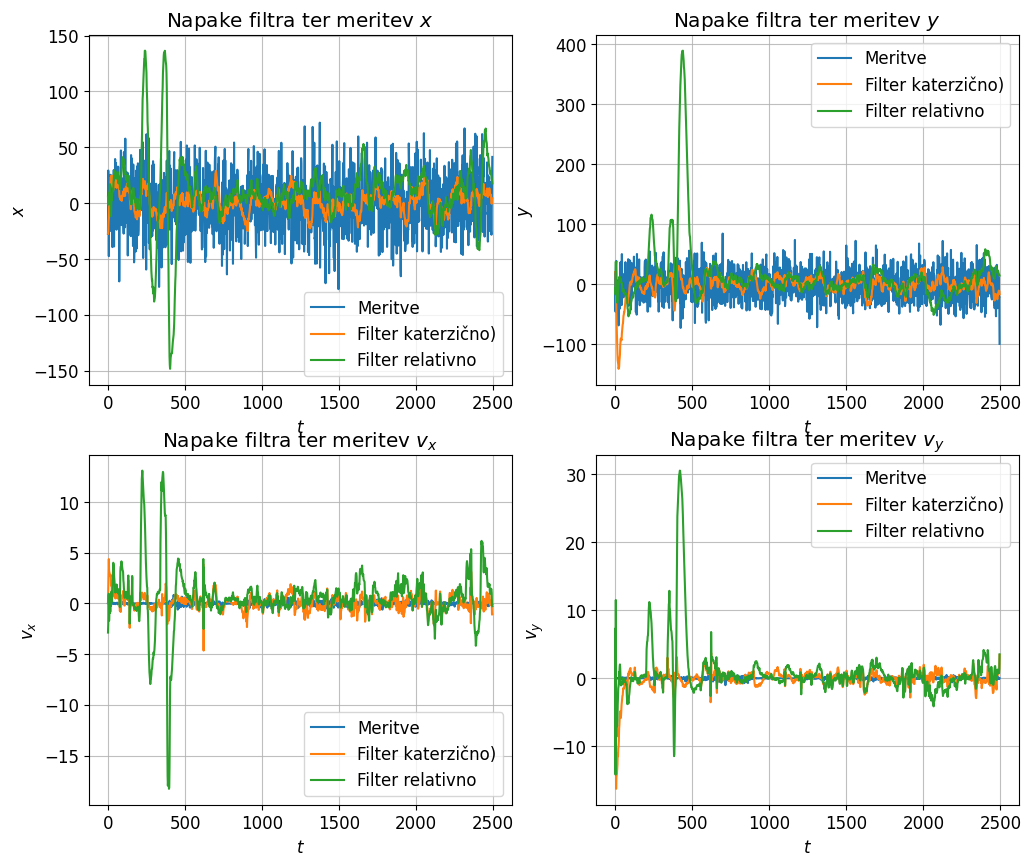
\includegraphics[width=14cm]{slika12.png}
\caption{Napake količin dobljenih s relativnim ter katerzičnim kKalmanovim filtrom v odvisnosti od časa.}
\end{figure}

Na sliki 13 vidimo celo, da so kovariance po določenem času praktično enake pri obeh filtrih.

\begin{figure}[h!]
\centering
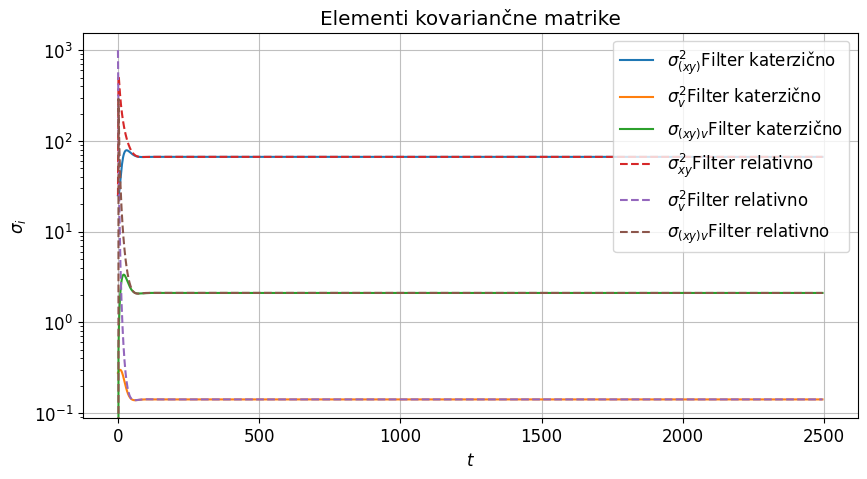
\includegraphics[width=12cm]{slika13.png}
\caption{Elementi kovariančne matrike $P^+$ za katerzični Kalmanov filter s polnimi črtami ter za relativni Kalmanov filter s črtkanimi črtami. Vidimo, da so kovariance filtrov po nekem času praktično enake.}
\end{figure}

\section{Zaključek}

V nalogi smo s Kalmanovim filtrom rekonstruirali pot od Ljubljane do Litije. Iz zašumljenih podatkov smo z optimalnim filtriranjem zgladili pot in dobili bolj realne rezultate. Raziskali smo kako dobro nastopa Kalmanov filter s podajanjem meritev o položaju ter hitrostmi, ter le eno izmed teh dveh. Prav tako smo sestavili Kalmanov filter za bolj realen primer, kjer pospeške merimo relativno in ne v laboratorijskem sistemu.

\end{document}